
% Introduction

The project initially was defined to be implementation of following article \cite{wordembedspeech}. The article in general has following approach: 
\begin{itemize}
    \item Build an end-to-end neural network to perform  speech to text 
    \item Create a feature scheme called letter-n-grams to convert a word into a fixed sized  vectors (long vectors)
    \item Train a neural network to map the letter-n-gram to the embedding layer of the main speech to text network 
\end{itemize}

The idea is quiet straight forward we want to have a function from letter-n-grams to a dense representation of the sound of the word.  This looks very interesting as it can help us to group the word that are sounding similar together. The is a useful function for performing search operation. Another interesting gain from this mapping is the fact that we can estimate on the words that are not in our  speech corpus. This can give us a good advantage to work with larger vocabularies compared to our original speech corpus. 


\begin{figure}[hbt!]
    \centering
    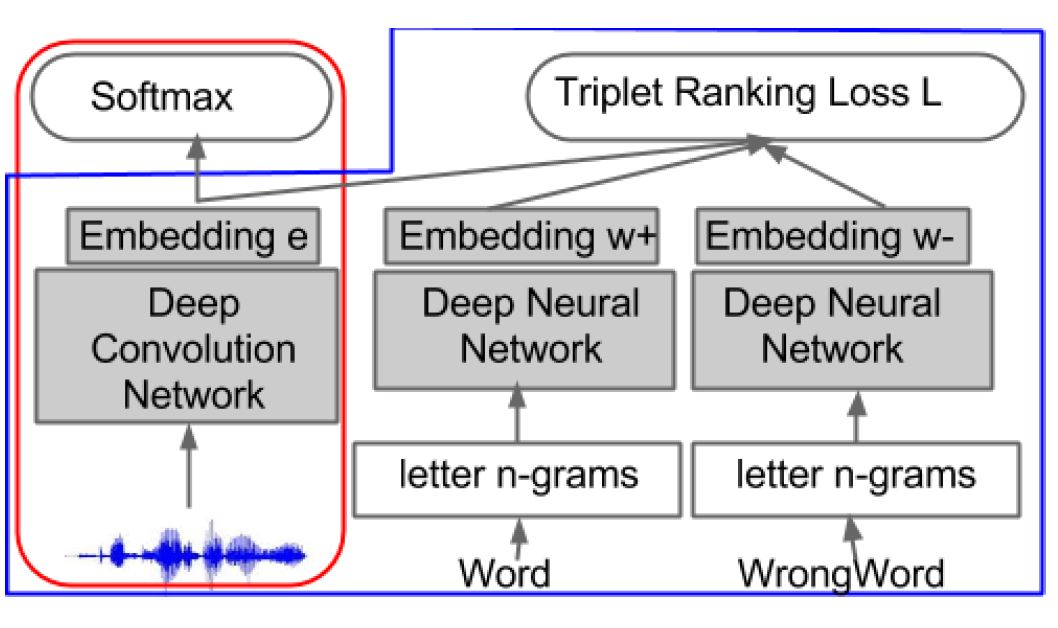
\includegraphics{Images/genera_model.jpg}    
    \caption{Main Approach in \cite{wordembedspeech} - The image is from the original article}
    \label{article_main_approach}
\end{figure}

\subsection{Implementation Challenge}
Although the logic of the article was clear but there were some challenges that made it impossible to directly implement what was in the article. We will going through these challenges. 
\begin{itemize}
    \item Dataset Challenge
    \item Computational Challenge 
    \item Some unspecified architectural parameters 
\end{itemize}

We will go through all of these challenges one by one.
\subsubsection{Dataset Challenge}
The dataset that is mentioned in the article is not publicly available. This gives us a big challenge on the getting corpus that can be used. It is stated in the article that some sort of private speech corpus been used.  Se we decided to use one of the open speech corpora available publicly. 

We used the LibriSpeech \cite{DBLP:conf/icassp/PanayotovCPK15}. This corpus is based on public domain audio books and is available publicly. We will provide detailed information about this corpus in later sections. 

\subsubsection{Computational Challenge}
In the article the authors try to build an end-to-end neural network for speech processing. Training such model is computationally very expensive. It has 8 fully connected layers which make it very hard to train. From what paper talks about a week of training for such network on GPU heavy machine. Whereas for baseline models it requires 100 machines with a week of time.  This was not something that is possible for us to handle within the time frame that we had. To overcome this challenge we were looking for a pre-trained model that already has done the complexity of training for us. We landed to use DeepSpeech model \cite{DBLP:journals/corr/HannunCCCDEPSSCN14} which is an open model based on tensor flow. Both code and pretrained model is available publicly. The plan became to tap into the code and do what we want on it. 
\subsubsection{Unclear Architecture}
The article is quiet clear about the architecture of the text-to-speech network. But unfortunately skips the important details about the layers, activation functions and connectivity of the layers. It only talks about the loss function of this network. This information is crucial for us to implement the model successfully. 

\subsection{Main Decision}
After dealing with above challenges, I decided to take a new but similar approach to what \cite{wordembedspeech} has proposed. The approach it keep the general idea of the article but implement it in a different way. In next section the proposed approach is being discussed. 